\documentclass{article}

% Math packages
\usepackage{amsmath}
\usepackage{amssymb}

% R Table packages
\usepackage{booktabs}
\usepackage{float}
\usepackage{colortbl}
\usepackage{xcolor}

% Page layout libraries
\usepackage{a4wide}
\usepackage{setspace}
\usepackage{geometry}
\usepackage{parskip}
\usepackage{fancyhdr}

% Setting up the heading style preferred here
\pagestyle{fancy}
\fancyhead[L]{\thepage}
\fancyhead[C]{}
\fancyhead[R]{\textrm{Robert Petit}}
\fancyfoot[L, C, R]{}


% this package helps us with including images. Setting the graphics path makes it easier to refer to things in the \includegraphics command.
\usepackage{graphicx}
\graphicspath{ {../figures/} }

% Titling
\title{Incarceration Analysis}
\author{Robert Petit}
\date{February, 2022}

\begin{document}
\maketitle

Using the NLSY97 data, we can investigate some information about incarcerations among the participants. The first notable trends show up when we simply look at the mean number of months spent incarcerated by race and gender, as seen in Figure \ref{fig:MeanMonths}. 

\begin{figure}[H]
    \begin{center}
        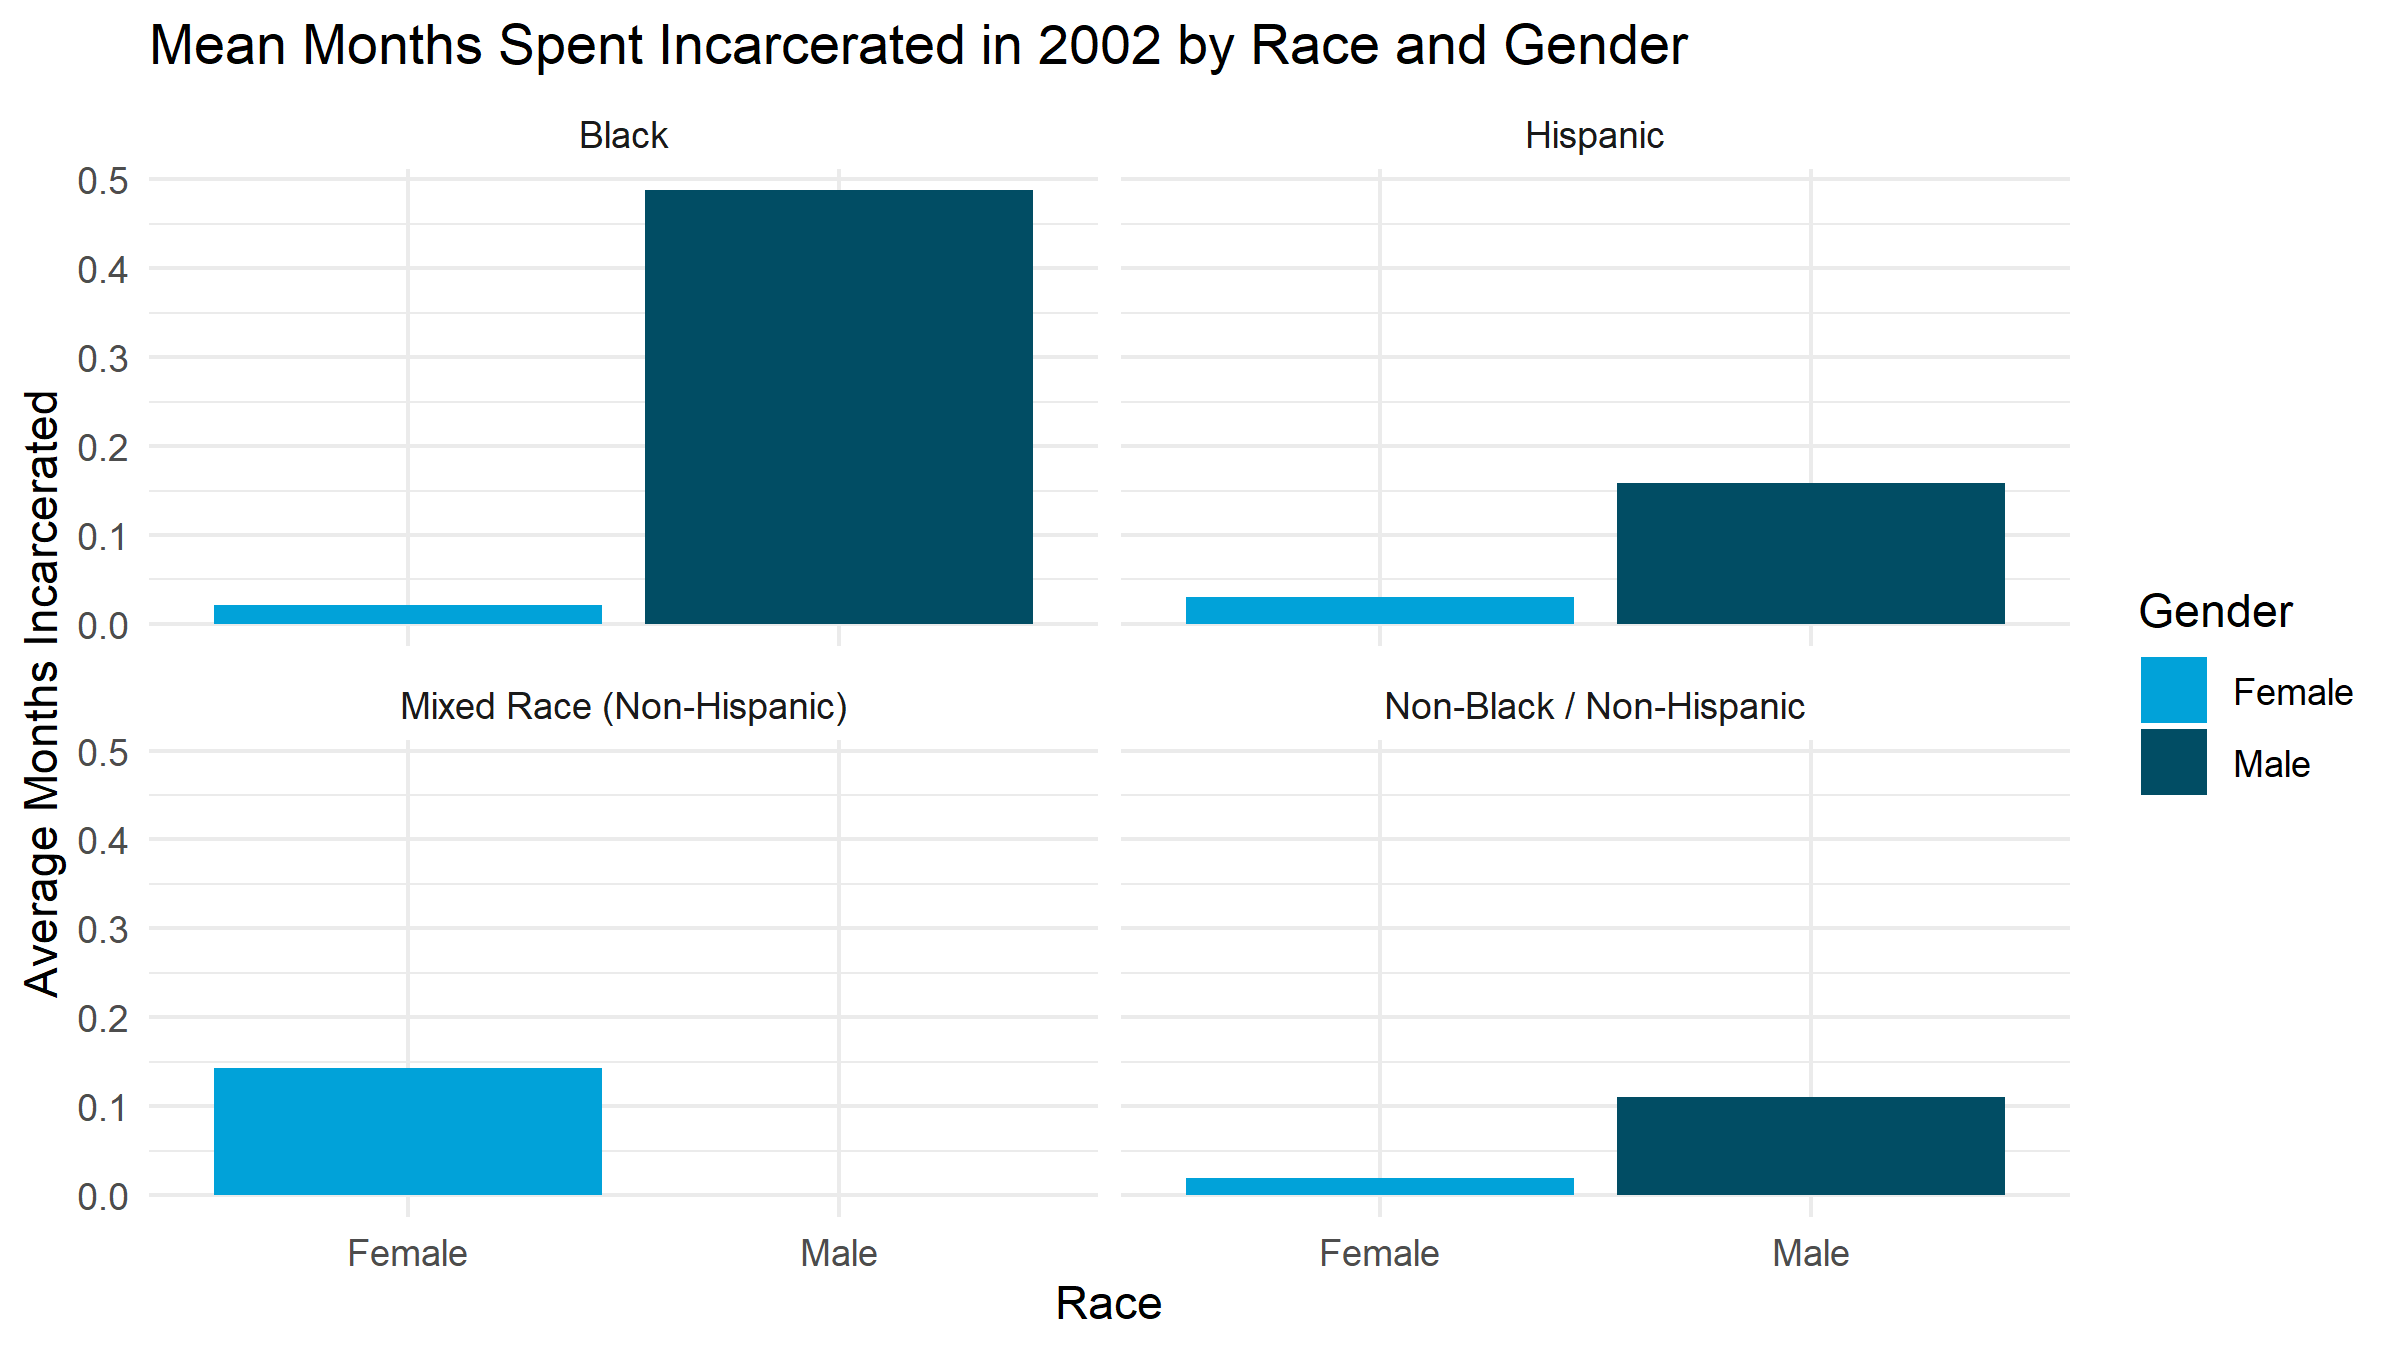
\includegraphics[width=.85\textwidth]{MonthsIncarcerated_by_racegender}
    \end{center}
    \caption{Months spent incarcerated, by race and gender}
    \label{fig:MeanMonths}
\end{figure}

These trends are not incredibly surprising, the number of months spent incarcerated during a year is dramatically higher for black males than any other combination of race and gender; it is more than triple that of the next highest category, seen more precisely in table  \ref{tab:summarystats}.

\begin{table}[H]

\caption{\label{tab:summarystats}Mean Months Incarcerated in 2002 by Race and Gender}
\centering
\begin{tabular}[t]{lrrrr}
\toprule
Gender & Black & Hispanic & Mixed Race Non Hispanic & Non Black Non Hispanic\\
\midrule
\cellcolor{gray!6}{Female} & \cellcolor{gray!6}{0.0211268} & \cellcolor{gray!6}{0.0298013} & \cellcolor{gray!6}{0.1428571} & \cellcolor{gray!6}{0.0193192}\\
Male & 0.4876712 & 0.1579509 & 0.0000000 & 0.1099476\\
\bottomrule
\end{tabular}
\end{table}


A very simple regression also gives some estimation of the magnitude of these effects.


% Table created by stargazer v.5.2.2 by Marek Hlavac, Harvard University. E-mail: hlavac at fas.harvard.edu
% Date and time: Fri, Feb 18, 2022 - 3:19:39 PM
\begin{table}[!htbp] \centering 
  \caption{Regression Output. Omitted category is Black Females.} 
  \label{tab:regression} 
\begin{tabular}{@{\extracolsep{5pt}}lc} 
\\[-1.8ex]\hline 
\hline \\[-1.8ex] 
 & \multicolumn{1}{c}{\textit{Dependent variable:}} \\ 
\cline{2-2} 
\\[-1.8ex] & Months Incarcerated in 2002 \\ 
\hline \\[-1.8ex] 
 Hispanic & $-$0.159$^{***}$ \\ 
  & (0.038) \\ 
  & \\ 
 Mixed Race (Non-Hispanic) & $-$0.174$^{**}$ \\ 
  & (0.083) \\ 
  & \\ 
 Non-Black / Non-Hispanic & $-$0.189$^{***}$ \\ 
  & (0.035) \\ 
  & \\ 
 Male & 0.194$^{***}$ \\ 
  & (0.022) \\ 
  & \\ 
 Constant & 0.155$^{***}$ \\ 
  & (0.026) \\ 
  & \\ 
\hline \\[-1.8ex] 
Observations & 8,621 \\ 
R$^{2}$ & 0.015 \\ 
Adjusted R$^{2}$ & 0.014 \\ 
Residual Std. Error & 1.019 (df = 8616) \\ 
F Statistic & 32.033$^{***}$ (df = 4; 8616) \\ 
\hline 
\hline \\[-1.8ex] 
\textit{Note:}  & \multicolumn{1}{r}{$^{*}$p$<$0.1; $^{**}$p$<$0.05; $^{***}$p$<$0.01} \\ 
\end{tabular} 
\end{table} 


Since black females are the omitted category, in order to understand the expectation of black males related to other combinations we have to observe the intercept and male coefficient simultaneously. As it turns out, these are the \emph{only} two positive coefficients which captures the information of the above graphs more accurately. It should also be noted that these values are all statistically significant to a high degree, with p-values less than 0.01.

Ultimately, this data is very consistent with the common understanding of incarceration in the US. It varies significantly and consistently based on race. It should be notes that these are all correlational observations, and making a causal claim requires more complex observations.

\end{document}